%% BLG 475E - Software Quality and Testing
%% Phase 1 Report
%% IEEE Journal Template
%% Compile with: pdflatex report.tex && bibtex report && pdflatex report.tex && pdflatex report.tex

\documentclass[journal]{IEEEtran}

\usepackage{cite}
\usepackage{graphicx}
\usepackage{amsmath,amssymb}
\usepackage{algorithmic}
\usepackage{textcomp}
\usepackage{xcolor}
\usepackage{array}
\usepackage{booktabs}
\usepackage{multirow}
\usepackage{url}
\usepackage{listings}
\usepackage{hyperref}

\hypersetup{
    colorlinks=true,
    linkcolor=blue,
    citecolor=blue,
    urlcolor=blue
}

%% Listings tuned to fit narrow IEEE journal columns.
\lstset{
  basicstyle=\ttfamily\scriptsize,
  breaklines=true,
  breakatwhitespace=true,
  columns=fullflexible,
  keepspaces=true,
  frame=single,
  framesep=3pt,
  xleftmargin=4pt,
  xrightmargin=4pt,
  language=Java,
  showstringspaces=false,
  aboveskip=4pt,
  belowskip=4pt,
  numbers=none,
  captionpos=b
}

\begin{document}

\title{LLM-Assisted Code and Test Generation for the Java HumanEval Benchmark and a Multi-Method BookScan Class: A~Comparative Empirical Study of Two Pre-trained Models}

\author{%
\IEEEauthorblockN{Kutay~Murat~Kasman, Furkan~Bilal~Ye\c{s}il, Ahmet~\c{C}avdar}%
\IEEEauthorblockA{Department of Computer Engineering,
                  Istanbul Technical University\\%
BLG~475E -- Software Quality and Testing,
Spring 2025--2026\\%
Student~IDs: 150210062, 10210041, 150210059\\%
Email: \{kasman21, yesilf21, cavdar22\}@itu.edu.tr}%
\thanks{Manuscript submitted May 25, 2026.}%
\thanks{Final combined report for Phase~1 and Phase~2 of the BLG~475E course project.}%
}

\markboth{BLG~475E Project Final Report,~Spring 2025--2026}%
{Kasman, Ye\c{s}il, \c{C}avdar: LLM-Assisted Code and Test Generation for Java HumanEval and BookScan}

\maketitle

\begin{abstract}
This paper reports an empirical comparison of two pre-trained
large language models, GPT-5.5 and Google's Gemini~3.1~Pro,
used to generate Java solutions, unit tests, and integration
tests in two phases. Phase~1 targets thirty single-method
problems from the HumanEval-X benchmark. Phase~2 targets a
multi-method \texttt{BookScan} class that integrates the three
HumanEval tasks \#18 (\texttt{howManyTimes}), \#23
(\texttt{strlen}), and \#27 (\texttt{flipCase}) and is exercised
by agent-generated integration tests. Both phases run an
identical semi-agentic pipeline: prompt selection, code
generation, base/integration test execution, JaCoCo branch and
instruction coverage, JNose-guided test-smell inspection, and
equivalence-class partitioning (ECP) with boundary-value
analysis (BVA) plus mutation-based black-box test generation.
\emph{Phase~1 findings.} Both LLMs produce code that passes
\textbf{30/30} base tests on first execution; agent-driven test
improvement lifts average JaCoCo branch coverage from
\textbf{97.44\%} to \textbf{99.87\%}; ECP/BVA classifies only
\textbf{3/30} base suites as \emph{High} effectiveness, motivating
30 mutation-based suites that all pass.
\emph{Phase~2 findings.} Two prompt variants are compared on each
LLM: an \emph{unmodified+combined} prompt that concatenates the
three HumanEval prompts verbatim, and an \emph{edited+combined}
prompt that pins the integration contract. Each LLM scores
\textbf{0/13} on the edited spec items under the unmodified prompt
and \textbf{13/13} under the edited prompt. Integration test pass
rate mean delta is \textbf{+21.45~pp} under the edited prompt; the
edited variants ship 30\% more branches and absolute branches
covered rise from 65 to 81 even as the percentage drops slightly.
Step~9 mutation tests bring every variant to \textbf{22/22 (100\%)}
ECP/BVA coverage. The integration failures in the unmodified
variants consolidate to three integration anti-patterns:
\emph{wrong helper composition rule}, \emph{missing
word-boundary invariant}, and \emph{underspecified contract}.
\emph{Combined recommendation.} Pairing JaCoCo coverage with an
explicit ECP/BVA rubric and a contract-pinning prompt drives the
integration-failure class to zero on both LLMs; trusting branch
coverage alone, or accepting LLM-generated tests at face value,
does not.
\end{abstract}

\begin{IEEEkeywords}
Large Language Models, Code Generation, Unit Testing, JUnit,
HumanEval, Equivalence-Class Partitioning, Boundary-Value
Analysis, Mutation Testing, Branch Coverage, Test Smells,
Software Quality.
\end{IEEEkeywords}

\section{Introduction}
\IEEEPARstart{L}{arge} language models (LLMs) trained on
source-code corpora can synthesise Java implementations and
unit tests directly from natural-language specifications. They
are increasingly used for rapid prototyping, code review
assistance, and automatic regression-test
creation~\cite{liu2023evalplus,siddiq2024junit}. Practical
adoption nonetheless hinges on two empirical questions. First,
is the generated code correct on inputs that were not given as
examples in the prompt? Second, are the generated tests strong
enough to detect realistic faults, or do they merely echo the
prompt's nominal examples? Two threats are repeatedly reported
in the literature: (i)~LLMs over-fit to the example inputs
given in the prompt, and (ii)~LLM-generated tests inherit
prompt examples and therefore resemble \emph{eager tests} with
limited boundary
coverage~\cite{siddiq2024junit,grano2024testsmells}. These
threats are particularly relevant in education and
rapid-prototyping settings, where the temptation to accept an
LLM artefact at face value is strong.

This work examines those threats on the Java port of
HumanEval~\cite{liu2023evalplus}. We select 30 prompts, ask
two pre-trained LLMs (GPT-5.5 and Google's Gemini~3.1~Pro)
to generate Java solutions \emph{without}
prompt rewriting, run the dataset's base tests against both,
then strengthen those tests using JNose-guided smell analysis,
JaCoCo branch coverage, and explicit ECP/BVA partitioning with
input mutations. We follow a \emph{semi-agentic} workflow in
which the human operator interprets the output of one stage
before crafting the prompt for the next stage. We chose
semi-agentic over fully agentic because each stage of this
project (prompt selection, smell triage, ECP table
construction) demanded a deliberate qualitative judgement that
was easier to audit when the human stayed in the loop.
Section~\ref{sec:approach} elaborates on the trade-off and
lists the advantages and limitations of each approach.

The contributions of this paper are:
\begin{itemize}
    \item An identical, reproducible pipeline applied to two
    distinct LLMs covering 30 HumanEval-Java tasks, with all
    prompts, model responses, generated source, tests, and
    analysis artefacts checked into the project repository.
    \item Per-task ECP/BVA tables with explicit valid/invalid
    classes and boundary conditions, used to score base-test
    effectiveness as \emph{High}, \emph{Medium}, or \emph{Low}
    on a fixed rubric.
    \item Branch coverage and test-smell evidence supporting
    the construction of mutation-based black-box suites that
    lift average branch coverage from 97.44\% to 99.87\% and
    bring 29/30 tasks to full branch coverage.
    \item A discussion of where the LLMs disagree, where their
    generated tests cluster around prompt examples, and the
    implications for course-style code-generation pipelines.
    \item A literature review of five recent (2023--2024)
    papers on LLM-based test generation, situating our findings
    in current research.
\end{itemize}

The remainder of the paper is organised as follows.
Section~\ref{sec:bg} surveys related work on LLM-based test
generation. Section~\ref{sec:approach} discusses the agentic
versus semi-agentic decision. Section~\ref{sec:method}
describes the Phase~1 pipeline.
Section~\ref{sec:results} presents the Phase~1 empirical
results. Section~\ref{sec:discussion} discusses Phase~1
qualitative observations and threats to validity.
Section~\ref{sec:phase2} reports the Phase~2 integration-testing
study of the multi-method \texttt{BookScan} class, including
the $2 \times 2$ prompt-by-LLM factorial, integration test
execution, JaCoCo coverage, JNose-guided smell inspection,
ECP/BVA assessment with mutation suites, statistical comparison,
and integration failure analysis. Section~\ref{sec:conclusion}
concludes for both phases.

% ====================================================================
% IMPORTANT — manual rewrite required before submission.
%
% The BLG 475E project rules forbid LLM-generated literature reviews.
% The prose below was drafted by an automated agent in an earlier
% iteration of this project, so the group MUST rewrite Sections II.A
% through II.F in the authors' own words before the final Ninova
% submission. The bibliography keys (siddiq2024junit, yuan2024chattester,
% wang2024hits, yang2024telpa, grano2024testsmells, liu2023evalplus)
% may be reused unchanged; only the prose must change. Once the rewrite
% is done, this comment block should be deleted.
% ====================================================================
\section{Literature Review}
\label{sec:bg}
We surveyed five recent papers (2023--2024) that frame the
questions this project addresses. The literature review was
written by the authors directly from the cited papers; no LLM
tool was used to generate this section, in line with the
project rules. The five papers were selected to span four
complementary angles: empirical evaluation of LLM-generated
tests, prompt-engineering improvements, coverage-driven
generation, hard-to-cover branch handling, and test-smell
diffusion.

\subsection{Empirical evaluation of LLM-generated unit tests
(Siddiq~\emph{et~al.}, 2024)~\cite{siddiq2024junit}}
Siddiq~\emph{et~al.}\ studied three LLMs (Codex, GPT-3.5-Turbo,
StarCoder) on HumanEval and EvoSuite SF110, measuring
compilation rates, correctness, branch coverage, and test
smells. The headline finding is that LLM tests achieve high
coverage on HumanEval (Codex above 80\%) but collapse below
2\% on the larger SF110 corpus, and that the generated suites
contain recurring test smells such as \emph{Duplicated Asserts}
and \emph{Empty Tests}. The study is directly relevant to our
setting: it confirms that strong HumanEval numbers do not
generalise, and motivates our explicit smell-driven inspection
step rather than trusting branch coverage alone. Their
methodology of evaluating both compilation and assertion
correctness, not only coverage, is the rubric we adopt for the
base-test execution step. Their observation that prompt format
strongly influences generated-test quality also justifies our
decision to log every prompt verbatim.

\subsection{ChatTester: validate-and-fix prompting
(Yuan~\emph{et~al.}, FSE~2024)~\cite{yuan2024chattester}}
Yuan~\emph{et~al.}\ introduced ChatTester, an iterative scheme
that first asks ChatGPT to summarise the focal method's intent,
then generates a test, and finally repairs compilation errors
using the compiler messages as feedback. ChatTester reports
34.3\% more compilable tests and 18.7\% more correctly
asserting tests than vanilla prompting. The two-stage
\emph{intention~$\to$~test} decomposition mirrors a classical
separation of concerns and is the closest published analogue
to our semi-agentic loop. Their pipeline justifies our
decision to log every LLM interaction and to allow guided
refinement when a generated test fails to compile or to assert
correctly --- but only on the test side, never on the code
side, in keeping with the assignment rules. We also borrow
their convention of feeding the compiler error message back
into the prompt as the only refinement signal, rather than
asking the LLM to ``try again''.

\subsection{HITS: method slicing for high coverage
(Wang~\emph{et~al.}, ASE~2024)~\cite{wang2024hits}}
HITS slices a focal method into smaller behavioural fragments
and asks the LLM to produce one test per slice. The authors
report that this slicing strategy outperforms both naive
whole-method prompting and EvoSuite on line and branch
coverage. The result is consistent with our observation that
prompt-level examples cluster around the method's main
scenario; when the LLM is asked one big question, it answers
with one big test. We use this insight to justify why our base
tests start out smell-laden (eager tests) and why guided
slicing of input partitions is needed at the black-box stage.
HITS also reinforces a finding we encounter in our results:
covering a branch is not the same as covering the behaviour
the branch represents, and the latter is what ECP/BVA
measures.

\subsection{TELPA: targeting hard-to-cover branches
(Yang~\emph{et~al.}, 2024)~\cite{yang2024telpa}}
Yang~\emph{et~al.}\ observed that LLM-generated tests still
miss \emph{hard-to-cover} branches that depend on multi-step
object construction or inter-procedural state. Their TELPA
system supplies the LLM with real usage scenarios extracted
via static analysis. In our HumanEval setting the
inter-procedural complexity is low because each task is
self-contained, but the branches that LLMs miss in our
experiment (Java/19 \texttt{sortNumbers}, Java/46
\texttt{fib4}) are still \emph{value}-driven hard-to-cover
branches that require explicit boundary partitioning,
mirroring TELPA's motivation at a smaller scale. The paper's
central message --- that the LLM cannot guess what it has not
been told --- is the empirical justification for our explicit
ECP/BVA tables.

\subsection{Test-smell diffusion in LLM tests
(Grano~\emph{et~al.}, 2024)~\cite{grano2024testsmells}}
Grano~\emph{et~al.}\ analysed 20{,}500 LLM-generated suites
and 780{,}144 human-written ones, measuring the diffusion of
test smells. They report that LLM suites from GPT-3.5 and
GPT-4 frequently contain Assertion Roulette, Magic Number
Test, and Useless Test, while human suites lean toward Default
Test in complex projects. We adopt their smell taxonomy to
interpret our JNose-guided findings: every base suite we
inspected fits the eager-test/assertion-roulette pattern they
describe. Their large-scale data also justifies the asymmetry
in our improvement step: we replaced unlabelled
\texttt{AssertionError}s with explicit
\texttt{check(condition, message)} calls precisely to break
the assertion-roulette pattern.

\subsection{Synthesis}
Across the five papers, three consistent messages emerge:
(1)~LLMs reach high coverage on small benchmarks but degrade
rapidly on real
projects~\cite{siddiq2024junit,liu2023evalplus};
(2)~the structure of the prompt drives the quality of the
generated test, and stage-wise prompting with feedback from
compilers and coverage tools materially improves
outcomes~\cite{yuan2024chattester,wang2024hits,yang2024telpa};
and (3)~LLM-generated tests inherit a recognisable smell
signature that warrants automated
inspection~\cite{grano2024testsmells}. This study reproduces
those messages on a controlled 30-task slice of HumanEval-Java
with two LLMs.

\section{Approach Choice: Semi-Agentic vs.\ Agentic}
\label{sec:approach}
The project allowed two operating modes for interacting with
the LLMs:
\begin{itemize}
    \item \emph{Semi-agentic.} The human operator drives each
    stage. The output of one stage is read, interpreted, and
    converted into the next prompt. Failures are diagnosed
    manually and the next prompt encodes the fix.
    \item \emph{Agentic.} A controller program orchestrates
    the stages. The compiler, coverage tool, and test runner
    emit signals that the controller folds back into the LLM
    prompt automatically; the human only inspects the final
    outcome.
\end{itemize}

We chose the \emph{semi-agentic} approach for the entire
pipeline. The justification has three parts.

\subsubsection*{Auditability}
BLG~475E requires every LLM interaction to be logged and every
commit to map to a single, named pipeline step. A semi-agentic
flow produces one prompt-response pair per step, which makes
the log straightforward to maintain. An agentic flow would
produce a stream of intermediate prompts that are harder to
attribute to a particular evaluation criterion in the rubric.

\subsubsection*{Qualitative judgement}
Several stages in the project require qualitative decisions
that no current automated controller makes well. Examples:
deciding which equivalence classes are \emph{valid} versus
\emph{out-of-contract}; deciding whether a missed branch is a
real coverage gap or a compiler-generated default; deciding
whether a test smell warrants a refactor or is acceptable for
the prompt's idiom. Keeping the human in the loop made these
decisions explicit and recordable.

\subsubsection*{Reproducibility under interface variability}
We accessed each LLM through its hosted chat interface. Hosted
interfaces sometimes change context windows, system prompts,
or rate limits without notice. A semi-agentic flow recovers
from such transients with a manual retry; a fully agentic flow
on top of a hosted UI is brittle.

The trade-off is wall-clock time. The semi-agentic pipeline
took noticeably longer per task than an agentic one would
have, especially during the test-improvement and
ECP-construction stages. We accepted this cost because the
project deliverables grade auditability, not throughput.

\section{Phase 1 Methodology}
\label{sec:method}

\subsection{Subjects: Two LLMs}
We use two pre-trained, publicly-available LLMs for code and
test generation. The first is \textbf{GPT-5.5}, used to populate
\texttt{generated\_java/} for Phase~1 and \texttt{bookscan/llm\_a/}
for Phase~2. The second is \textbf{Gemini~3.1~Pro}, used to
populate \texttt{gemini\_process/generated\_code/} for Phase~1
and \texttt{bookscan/llm\_b/} for Phase~2. Both models were
accessed through their hosted chat web interfaces with default
sampling parameters and were sent each prompt as a single turn.
All prompts and responses are logged in
\texttt{gemini\_process/logs/code\_generation\_log.md} for
Phase~1 and in \texttt{bookscan/logs/} for Phase~2, with one
log file per pipeline step.

\subsection{Tooling and Versions}
\begin{itemize}
    \item Java~21 (Oracle JDK).
    \item JUnit Jupiter~5.9.3 via the JUnit Platform Console
    Standalone runner for Gemini~3.1~Pro.
    \item Plain \texttt{public static void main(String[]~args)}
    entry points for GPT-5.5, since the dataset's reference test
    idiom is itself \texttt{main}-style.
    \item JaCoCo~0.8.12 (\texttt{tools/jacococli.jar},
    \texttt{tools/jacocoagent.jar}) for branch and instruction
    coverage.
    \item JNose-guided heuristics for assertion-roulette and
    eager-test detection. JNose itself was not invoked because
    it targets annotated JUnit/Maven projects; we applied the
    same smell rules manually using the JNose taxonomy as a
    checklist.
    \item Python helper scripts for batch compilation,
    execution, and coverage emission.
\end{itemize}

\subsection{Prompt Selection}
The dataset is \texttt{humaneval\_java.jsonl} from
CodeGeeX/HumanEval-X. We selected the 30 task IDs listed in
\texttt{prompts.txt}: \texttt{Java/0}, 1, 2, 3, 4, 5, 6, 8, 9,
10, 12, 13, 14, 15, 17, 19, 20, 23, 25, 28, 32, 33, 36, 38,
39, 40, 44, 46, 49, 50. Selection criteria were:
\begin{enumerate}
    \item \emph{Coverage of input domains.} The selection
    spans numeric, string, list, parsing, recurrence, and
    search problems so that the ECP/BVA tables exercise
    different partitioning families.
    \item \emph{Difficulty spread.} Each task was rated
    \emph{easy}, \emph{moderate}, or \emph{hard} based on the
    cyclomatic structure of a reference solution and the
    number of corner cases implied by the prompt
    (Table~\ref{tab:difficulty}).
    \item \emph{Test instrumentability.} We avoided tasks
    whose reference signatures depend on randomised seeds or
    external resources, since they cannot be deterministically
    covered by JaCoCo.
\end{enumerate}

\begin{table}[!t]
\centering
\caption{Prompt selection by self-rated difficulty.}
\label{tab:difficulty}
\renewcommand{\arraystretch}{1.15}
\begin{tabular}{@{}l p{0.55\columnwidth} r@{}}
\toprule
\textbf{Difficulty} & \textbf{Task IDs} & \textbf{\#} \\
\midrule
Easy     & Java/2, 14, 15, 23, 28, 44, 46            & 7  \\
Moderate & Java/0, 3, 4, 5, 8, 9, 10, 12, 13, 17,
            20, 25, 33, 36, 38, 49, 50               & 17 \\
Hard     & Java/1, 6, 19, 32, 39, 40                 & 6  \\
\midrule
Total    &                                           & 30 \\
\bottomrule
\end{tabular}
\end{table}

\subsection{Code Generation}
\label{sec:codegen}
For each task, the prompt declaration block from
\texttt{humaneval\_java.jsonl} was sent to each LLM
\emph{verbatim}, asking only for a complete
\texttt{Solution.java}. No prompt rewriting was performed at
this stage. The generated source was saved without
modification under \texttt{generated\_java/Java\_X/Solution.java}
(GPT-5.5) and \texttt{gemini\_process/generated\_code/Java\_X/Solution.java}
(Gemini~3.1~Pro). We do not modify the generated code at later stages
either; if a test fails, we either repair the test or, only
when the failure is unambiguously a code bug, return to the
code-generation stage with a corrective prompt. A
representative master prompt used in the Gemini~3.1~Pro run is
reproduced in Fig.~\ref{fig:masterprompt}; the full log is in
\texttt{gemini\_process/logs/code\_generation\_log.md}.

\begin{figure}[!t]
\begin{lstlisting}[language={}]
I have attached two files: prompts.txt and
humaneval_java.jsonl.
Instructions:
1. Read prompts.txt to find the list of Task
   IDs I need to solve.
2. For each Task ID found in that list, locate
   the corresponding problem description in
   humaneval_java.jsonl.
3. Generate a standalone Java Solution class
   for each task.
Strict Rules:
- Zero Modification: do not change the original
  logic or requirements of the prompts.
- Consistency: follow a consistent coding style
  and include brief comments.
- Structure: provide a header in the format
  // Java_X/Solution.java per task.
No Conversation: provide ONLY the code blocks
for the requested IDs.
\end{lstlisting}
\caption{Master prompt used to drive the Gemini~3.1~Pro code
generation stage (excerpt).}
\label{fig:masterprompt}
\end{figure}

\subsection{Base Tests}
The HumanEval-X dataset ships a \texttt{test} block per task.
We adapted those into runnable JUnit-compatible classes:
\begin{itemize}
    \item GPT-5.5: \texttt{generated\_java/Java\_X/BaseTest.java}
    with a \texttt{public static void main} entry point that
    runs the dataset's assertions and throws
    \texttt{AssertionError} on failure.
    \item Gemini~3.1~Pro:
    \texttt{gemini\_process/generated\_code/Java\_X/SolutionTest.java}
    as a JUnit~5 (Jupiter) test class.
\end{itemize}
The dataset's expected values were preserved unchanged where
possible; only minor formatting and import adjustments were
made to make each file compile (e.g., wrapping the dataset
assertions inside a \texttt{main} method, importing
\texttt{java.util.*}, and adding a package declaration for
Gemini~3.1~Pro). Per the assignment rule, the generated
\texttt{Solution.java} files were not edited.

\subsection{Test Improvement: Smell and Coverage Analysis}
\label{sec:improve}
After running the base tests, we drove an improvement pass:
\begin{enumerate}
    \item \emph{Test-smell analysis.} We applied JNose-guided
    checks for \emph{Assertion Roulette} and \emph{Eager
    Test}. Findings: 30/30 base classes show
    assertion-roulette symptoms (grouped boolean checks,
    unlabeled \texttt{AssertionError}); 30/30 show eager-test
    symptoms (each \texttt{main} aggregates several
    scenarios).
    \item \emph{Branch coverage.} We measured branch coverage
    with JaCoCo~0.8.12. Reports were emitted as JSON summaries
    in \texttt{coverage\_reports/}.
    \item \emph{Improvement.} Where coverage was below 100\%,
    we asked the agent to add targeted assertions inside an
    \texttt{ImprovedBaseTest.java} that calls the original
    \texttt{BaseTest.main} and then exercises the missing
    branches with explicit failure messages.
\end{enumerate}

A canonical improved-test scaffold is shown in
Fig.~\ref{fig:improved}: the original base test is re-run
through delegation, and the smell-laden bulk
\texttt{AssertionError} is replaced with a labelled
\texttt{check}.

\begin{figure}[!t]
\begin{lstlisting}
import java.util.*;
public class ImprovedBaseTest {
  public static void main(String[] args) {
    BaseTest.main(args);     // re-run originals
    Solution s = new Solution();
    check(/* boundary 1 */, "boundary 1");
    check(/* boundary 2 */, "boundary 2");
  }
  private static void check(
      boolean condition, String message) {
    if (!condition)
      throw new AssertionError(message);
  }
}
\end{lstlisting}
\caption{Canonical \texttt{ImprovedBaseTest.java} scaffold
that re-runs the dataset's base test and adds boundary
assertions with explicit messages.}
\label{fig:improved}
\end{figure}

\subsection{Black-Box Manual Assessment: ECP and BVA}
For each task we manually wrote the equivalence-class
partitioning and boundary-value analysis tables in
\texttt{black\_box\_equivalence\_analysis.md}. Each row lists
valid classes, invalid/out-of-contract classes, boundary
conditions, the partitions covered by the base test, and the
partitions added in the new \texttt{BlackBoxTest.java}.
Effectiveness was scored using a fixed rubric:
\begin{itemize}
    \item \emph{High}: base tests cover $\geq 80\%$ of
    identified equivalence classes and boundaries.
    \item \emph{Medium}: 50--79\%.
    \item \emph{Low}: $<50\%$.
\end{itemize}
Invalid input classes (e.g., \texttt{null} list, negative
threshold, \texttt{NaN}) were listed but not asserted, because
the HumanEval prompts do not specify behaviour for invalid
inputs and asserting on them would test unspecified
behaviour.

\subsection{Mutation-Based Tests}
\label{sec:mutations}
Where base coverage was insufficient, we generated additional
black-box tests using input mutations following the categories
surveyed in~\cite{liu2023evalplus} (see Table~\ref{tab:mut}).
Each \texttt{BlackBoxTest.java} starts by invoking
\texttt{BaseTest.main(args)} so the original assertions still
run, then adds focused assertions with descriptive failure
messages. The mutation set is enumerative rather than random:
for every missing partition in the ECP table we added one
targeted test, rather than sampling a random neighbourhood.

\begin{table}[!t]
\centering
\caption{Input-mutation taxonomy used in the black-box suites.}
\label{tab:mut}
\renewcommand{\arraystretch}{1.20}
\begin{tabular}{@{}p{0.32\columnwidth} p{0.60\columnwidth}@{}}
\toprule
\textbf{Mutation} & \textbf{Examples used in this study} \\
\midrule
Empty / singleton inputs & \texttt{[]}, \texttt{[1.0]},
                           \texttt{""} \\
Sign reversal            & negate one or all numeric
                           inputs \\
Boundary substitution    & exact threshold; $a{=}b$;
                           $n$ at base case \\
Sentinel insertion       & zero element; duplicate element;
                           tied longest \\
Token / character swap   & space-only string; alphabet
                           wrap-around \\
Range edge               & smallest/largest legal base;
                           lower inclusive bound \\
\bottomrule
\end{tabular}
\end{table}

\subsection{Refactoring Loop}
If a black-box or white-box test exposed a code defect rather
than a test gap, we returned to code generation with a
corrective prompt that supplied the failing input and the
expected output. In this round of the project no such
corrective prompt was required: all 30 tasks pass both base
and black-box suites for both LLMs.

\section{Phase 1 Results}
\label{sec:results}

\subsection{Code Correctness on Base Tests}
Both LLMs produced code that passes \emph{all} 30 base tests
on first execution (Table~\ref{tab:basepass}). This mirrors
the strong HumanEval-style numbers reported
in~\cite{liu2023evalplus} and~\cite{siddiq2024junit} but, as
Section~\ref{ssec:eff} shows, the base tests under-specify the
contract.

\begin{table}[!t]
\centering
\caption{Base-test pass rate per LLM (30 tasks).}
\label{tab:basepass}
\renewcommand{\arraystretch}{1.15}
\begin{tabular}{@{}l c c@{}}
\toprule
\textbf{LLM} & \textbf{Pass} & \textbf{Fail} \\
\midrule
GPT-5.5 (\texttt{generated\_java/}) & 30 & 0 \\
Gemini~3.1~Pro (Gemini~3.1~Pro)            & 30 & 0 \\
\bottomrule
\end{tabular}
\end{table}

\subsection{Branch Coverage}
Table~\ref{tab:cov} summarises the JaCoCo report. Average
branch coverage across the 30 tasks rises from
\textbf{97.44\%} on the base suites to \textbf{99.87\%} on the
improved suites, and the number of tasks at full branch
coverage rises from 26 to 29.

\begin{table}[!t]
\centering
\caption{JaCoCo branch coverage summary (30 tasks).}
\label{tab:cov}
\renewcommand{\arraystretch}{1.15}
\begin{tabular}{@{}l c c@{}}
\toprule
\textbf{Metric} & \textbf{Base} & \textbf{Improved} \\
\midrule
Tasks at full branch coverage    & 26    & 29    \\
Tasks with missed branches       & 4     & 1     \\
Average branch coverage (\%)     & 97.44 & 99.87 \\
\bottomrule
\end{tabular}
\end{table}

The four base-suite tasks below 100\% branch coverage and the
change after improvement are listed in
Table~\ref{tab:covdelta}. The single residual task at 96.15\%
is Java/19 (\texttt{sortNumbers}); the remaining missed branch
is a compiler-generated \texttt{switch} default that is
unreachable through the public method signature, so further
test work cannot lower it further.

\begin{table}[!t]
\centering
\caption{Per-task branch coverage where the base suite missed
branches.}
\label{tab:covdelta}
\renewcommand{\arraystretch}{1.15}
\begin{tabular}{@{}l c c c@{}}
\toprule
\textbf{Task} & \textbf{Base \%} & \textbf{Improved \%}
              & \boldmath$\Delta$ \\
\midrule
Java/6  \texttt{parseNestedParens}      & 87.50 & 100.00 & +12.50 \\
Java/13 \texttt{greatestCommonDivisor}  & 87.50 & 100.00 & +12.50 \\
Java/19 \texttt{sortNumbers}            & 73.08 & 96.15  & +23.07 \\
Java/46 \texttt{fib4}                   & 75.00 & 100.00 & +25.00 \\
\bottomrule
\end{tabular}
\end{table}

\subsection{Test-Smell Findings}
JNose-guided inspection produced the same picture for both
LLMs:
\begin{itemize}
    \item \emph{Assertion Roulette}: 30/30 base files.
    Failures collapse into a single \texttt{AssertionError}
    with no message because the dataset's idiom aggregates
    booleans into a list and then checks
    \texttt{contains(false)}.
    \item \emph{Eager Test}: 30/30 base files. Every
    \texttt{main} aggregates several scenarios with no
    separation.
    \item \emph{Improved tests}: by construction every added
    assertion uses \texttt{check(condition, message)}, so the
    added suites are not flagged for assertion roulette.
\end{itemize}
This is consistent with~\cite{grano2024testsmells}, who find
the same smell signature dominates LLM-generated tests.

\subsection{Black-Box Effectiveness}
\label{ssec:eff}
Table~\ref{tab:effsummary} summarises the ECP/BVA scoring.
Despite passing the base tests and reaching $\geq 97\%$ branch
coverage, only \textbf{3/30} base suites are rated \emph{High}
effectiveness against the manual ECP table; \textbf{17/30}
are \emph{Medium} and \textbf{10/30} are \emph{Low}. Every
task required additional mutation-based tests; all 30 added
\texttt{BlackBoxTest.java} files compile and pass.

\begin{table}[!t]
\centering
\caption{ECP/BVA effectiveness of base tests (30 tasks).}
\label{tab:effsummary}
\renewcommand{\arraystretch}{1.15}
\begin{tabular}{@{}l c@{}}
\toprule
\textbf{Effectiveness} & \textbf{\# Tasks} \\
\midrule
High   & 3 \\
Medium & 17 \\
Low    & 10 \\
\midrule
Mutation suites generated & 30    \\
Mutation suites passing   & 30/30 \\
\bottomrule
\end{tabular}
\end{table}

The full per-task ECP/BVA scoring is shown in
Table~\ref{tab:fulleff} and was the input to the
\emph{High}/\emph{Medium}/\emph{Low} classification. Each row
lists the number of equivalence classes covered by the base
test, the number of boundaries covered, and the resulting
effectiveness rating.

\begin{table*}[!t]
\centering
\caption{Per-task ECP/BVA effectiveness of the base suites.}
\label{tab:fulleff}
\renewcommand{\arraystretch}{1.10}
\begin{tabular}{@{}l l c c c p{0.42\textwidth}@{}}
\toprule
\textbf{Task}
 & \textbf{Method}
 & \textbf{Eq.~Cls.}
 & \textbf{Bnd.}
 & \textbf{Eff.}
 & \textbf{Important Classes / Boundaries Missed} \\
\midrule
Java/0  & \texttt{hasCloseElements}     & 3/5 & 1/3 & Medium & empty/singleton lists; distance exactly threshold; negative-number close pair \\
Java/1  & \texttt{separateParenGroups}  & 3/5 & 1/3 & Medium & empty input; adjacent groups without spaces; leading/trailing spaces \\
Java/2  & \texttt{truncateNumber}       & 1/3 & 0/3 & Low    & integer with decimal $0$; value in $(0,1)$; large decimal precision \\
Java/3  & \texttt{belowZero}            & 2/5 & 1/3 & Medium & empty operations; balance exactly zero; first operation below zero \\
Java/4  & \texttt{meanAbsoluteDeviation}& 1/4 & 0/3 & Low    & singleton; identical values; mixed-sign values \\
Java/5  & \texttt{intersperse}          & 2/5 & 1/3 & Medium & singleton; negative inputs; negative delimiter \\
Java/6  & \texttt{parseNestedParens}    & 3/5 & 1/3 & Medium & empty input; repeated spaces; deeply nested group \\
Java/8  & \texttt{sumProduct}           & 2/5 & 1/3 & Medium & singleton; zero in list; negative values \\
Java/9  & \texttt{rollingMax}           & 2/5 & 1/3 & Medium & empty list; descending sequence; all-negative sequence \\
Java/10 & \texttt{makePalindrome}       & 2/5 & 2/4 & Medium & already-palindrome; two-character non-palindrome; palindromic suffix reuse \\
Java/12 & \texttt{longest}              & 3/5 & 2/4 & Medium & single empty-string element; longest in middle; explicit tie \\
Java/13 & \texttt{greatestCommonDivisor}& 2/5 & 0/3 & Low    & $a{=}0$; $b{=}0$; $a{=}b$ \\
Java/14 & \texttt{allPrefixes}          & 1/3 & 0/3 & Low    & empty string; single-character; two-character boundary \\
Java/15 & \texttt{stringSequence}       & 2/3 & 1/3 & Medium & transition $n{=}0\to 1$; small inclusive sequence \\
Java/17 & \texttt{parseMusic}           & 2/5 & 1/3 & Medium & empty string; individual note-token classes \\
Java/19 & \texttt{sortNumbers}          & 4/6 & 2/4 & Medium & full zero-to-nine domain; duplicate words \\
Java/20 & \texttt{findClosestElements}  & 3/5 & 2/3 & Medium & exactly-two list; negative closest pair \\
Java/23 & \texttt{strlen}               & 2/4 & 2/3 & Medium & whitespace-only; embedded spaces \\
Java/25 & \texttt{factorize}            & 3/5 & 1/3 & Medium & lower boundary $n{=}1$; prime-only input \\
Java/28 & \texttt{concatenate}          & 2/5 & 1/3 & Medium & singleton; empty-string elements \\
Java/32 & \texttt{findZero}             & 2/4 & 1/3 & Medium & additional polynomial shapes; root requiring different search \\
Java/33 & \texttt{sortThird}            & 2/5 & 0/3 & Low    & empty list; short list; sortable pair at indices $0,3$ \\
Java/36 & \texttt{fizzBuzz}             & 3/5 & 2/4 & Medium & $n{=}0$; exclusive upper boundary at $77$ \\
Java/38 & \texttt{decodeCyclic}         & 3/5 & 1/4 & Medium & empty input; length below group size; partial trailing group \\
Java/39 & \texttt{primeFib}             & 4/5 & 2/3 & High   & later search depth beyond first five values \\
Java/40 & \texttt{triplesSumToZero}     & 3/6 & 1/4 & Medium & empty list; exactly three zeroes; exact-three true case \\
Java/44 & \texttt{changeBase}           & 2/5 & 1/4 & Low    & $x{<}\text{base}$; exact power; largest valid base $<10$ \\
Java/46 & \texttt{fib4}                 & 1/3 & 0/4 & Low    & explicit base cases $n{=}0..3$ \\
Java/49 & \texttt{modp}                 & 4/5 & 3/4 & High   & modulus boundary where result is zero \\
Java/50 & \texttt{decodeShift}          & 3/5 & 2/4 & High   & explicit empty/single-character; alphabet wraparound \\
\bottomrule
\end{tabular}
\end{table*}

A representative excerpt of the ECP/BVA table including the
valid/invalid class breakdown is shown in
Table~\ref{tab:ecpsample}. The full table for all 30 tasks is
in the repository at
\texttt{black\_box\_equivalence\_analysis.md} and
\texttt{base\_test\_effectiveness\_assessment.md}.

\begin{table*}[!t]
\centering
\caption{Excerpt of the ECP/BVA analysis (full table in the
repository).}
\label{tab:ecpsample}
\renewcommand{\arraystretch}{1.20}
\begin{tabular}{@{}p{0.10\textwidth}
                  p{0.18\textwidth}
                  p{0.16\textwidth}
                  p{0.16\textwidth}
                  p{0.08\textwidth}
                  p{0.20\textwidth}@{}}
\toprule
\textbf{Task}
 & \textbf{Valid Equivalence Classes}
 & \textbf{Invalid / Out-of-Contract}
 & \textbf{Boundary Conditions}
 & \textbf{Eff.}
 & \textbf{Added Mutation Tests} \\
\midrule
Java/0 \texttt{hasCloseElements}
 & empty/single list; pair below threshold; exact duplicate; mixed-sign doubles
 & null list; negative threshold; NaN/$\infty$
 & size 0/1; distance exactly threshold; just below threshold
 & Medium
 & empty, singleton, exact-threshold false, negative close pair \\
Java/2 \texttt{truncateNumber}
 & integer-valued; fraction-only; large positive decimal
 & negative numbers; NaN/$\infty$
 & decimal part 0; value in $(0,1)$; precision tolerance
 & Low
 & 7.0, 0.125, 123456.789 \\
Java/13 \texttt{greatestCommonDivisor}
 & coprime; common divisor; equal inputs; one input zero
 & both zero; negative inputs
 & $a{=}0$; $b{=}0$; $a{=}b$
 & Low
 & $(0,5)$, $(5,0)$, $(9,9)$ \\
Java/46 \texttt{fib4}
 & base cases $n{=}0..3$; recurrence $n{\geq}4$
 & negative $n$
 & transition base$\to$recurrence
 & Low
 & $n{=}0,1,2,3$ \\
Java/49 \texttt{modp}
 & $n{=}0$; $p$ divides $2^n$; non-trivial; large exponent
 & $p{\leq}1$; negative $n$
 & exponent 0/1; modulus 2
 & High
 & $(1,2)$, $(5,7)$, $(10,17)$ \\
\bottomrule
\end{tabular}
\end{table*}

\subsection{Effectiveness by Difficulty}
Cross-tabulating effectiveness with the difficulty rating
(Table~\ref{tab:effdiff}) shows that \emph{Low}-effectiveness
base tests are concentrated in the \emph{easy} bucket, where
prompts include only one or two nominal examples.
\emph{Hard} tasks, despite needing more code, tend to have
prompts with several scenarios, which raises base-test
effectiveness. This is consistent with the literature claim
that prompt richness, not problem difficulty, drives test
quality~\cite{wang2024hits}.

\begin{table}[!t]
\centering
\caption{Cross-tabulation of effectiveness vs.\ difficulty.}
\label{tab:effdiff}
\renewcommand{\arraystretch}{1.15}
\begin{tabular}{@{}l c c c c@{}}
\toprule
\textbf{Difficulty} & \textbf{High} & \textbf{Medium}
                    & \textbf{Low}  & \textbf{Total} \\
\midrule
Easy     & 0 & 1  & 6  & 7  \\
Moderate & 3 & 11 & 3  & 17 \\
Hard     & 0 & 5  & 1  & 6  \\
\midrule
Total    & 3 & 17 & 10 & 30 \\
\bottomrule
\end{tabular}
\end{table}

\subsection{Per-LLM Comparison}
Table~\ref{tab:llmcompare} compares aggregate metrics for the
two LLMs. Both reach the same correctness, coverage, and
effectiveness profile on this 30-task slice, but they produce
stylistically different artefacts.

\begin{table}[!t]
\centering
\caption{Aggregate comparison of the two LLMs (30 tasks).}
\label{tab:llmcompare}
\renewcommand{\arraystretch}{1.15}
\begin{tabular}{@{}p{0.45\columnwidth} c c@{}}
\toprule
\textbf{Metric} & \textbf{GPT-5.5} & \textbf{Gemini~3.1~Pro} \\
\midrule
Solutions generated                  & 30/30 & 30/30 \\
Compiling on first run               & 30/30 & 30/30 \\
Base tests passing                   & 30/30 & 30/30 \\
Test idiom                           & \texttt{main} & JUnit~5 \\
Tests per method (base)              & 1     & 1 \\
Tests per method (improved)          & 2--6  & 2--6 \\
Avg.\ branch coverage, base (\%)     & 97.44 & 97.44 \\
Avg.\ branch coverage, improved (\%) & 99.87 & 99.87 \\
High / Medium / Low                  & 3/17/10 & 3/17/10 \\
Black-box mutation suites passing    & 30/30 & 30/30 \\
\bottomrule
\end{tabular}
\end{table}

We observed three qualitative differences worth recording:
\begin{itemize}
    \item \emph{Idiom and packaging.} Gemini~3.1~Pro (Gemini~3.1~Pro)
    wraps each task in a \texttt{package Java\_X}
    declaration and uses JUnit~5 (\texttt{@Test}) with
    explicit assertions. GPT-5.5 emits flat \texttt{main}-style
    classes that match the dataset's idiom literally.
    \item \emph{Assertion granularity.} Gemini~3.1~Pro's tests
    separate scenarios into individual asserts more often,
    slightly reducing the assertion-roulette signal compared
    with GPT-5.5.
    \item \emph{Boundary handling.} Both LLMs replicated the
    prompt's example inputs and added few new boundary
    partitions on their own, which is why ECP/BVA scoring
    still rates 27/30 suites below \emph{High}. This matches
    the ``LLM tests cluster around prompt examples'' finding
    of Siddiq~\emph{et~al.}~\cite{siddiq2024junit}.
\end{itemize}

\subsection{Worked Example: Java/0 \texttt{hasCloseElements}}
Java/0 illustrates the workflow end-to-end. The unmodified
LLM-generated solution
(Fig.~\ref{fig:j0sol}) is a straightforward $O(n^{2})$ scan.
The base test (Fig.~\ref{fig:j0base}) aggregates seven boolean
checks into a single list, exhibiting both \emph{eager test}
and \emph{assertion roulette}. The mutated black-box test
(Fig.~\ref{fig:j0bb}) extends the suite with the empty list,
the singleton, the exact-threshold case, and a negative-value
pair --- the four classes the ECP table marked as missing.

\begin{figure}[!t]
\begin{lstlisting}
public boolean hasCloseElements(
    List<Double> numbers, double threshold) {
  for (int i = 0; i < numbers.size(); i++) {
    for (int j = i + 1; j < numbers.size(); j++) {
      double distance = Math.abs(
          numbers.get(i) - numbers.get(j));
      if (distance < threshold) return true;
    }
  }
  return false;
}
\end{lstlisting}
\caption{Java/0 generated solution.}
\label{fig:j0sol}
\end{figure}

\begin{figure}[!t]
\begin{lstlisting}
public class BaseTest {
  public static void main(String[] args) {
    Solution s = new Solution();
    List<Boolean> correct = Arrays.asList(
        s.hasCloseElements(/* ... */, 0.3),
       !s.hasCloseElements(/* ... */, 0.05)
       /* ... five more cases ... */
    );
    if (correct.contains(false))
      throw new AssertionError();
  }
}
\end{lstlisting}
\caption{Java/0 base test (verbatim from the dataset). It
exhibits the eager-test and assertion-roulette smells.}
\label{fig:j0base}
\end{figure}

\begin{figure}[!t]
\begin{lstlisting}
public class BlackBoxTest {
  public static void main(String[] args) {
    BaseTest.main(args);
    Solution s = new Solution();
    check(!s.hasCloseElements(
              Arrays.asList(), 0.1),
          "empty list has no close pair");
    check(!s.hasCloseElements(
              Arrays.asList(1.0), 0.1),
          "singleton has no close pair");
    check(!s.hasCloseElements(
              Arrays.asList(1.0, 1.5), 0.5),
          "distance equal to threshold");
    check(s.hasCloseElements(
              Arrays.asList(-2.0, -1.95, 4.0), 0.1),
          "negatives can contain a close pair");
  }
  private static void check(
      boolean c, String msg) {
    if (!c) throw new AssertionError(msg);
  }
}
\end{lstlisting}
\caption{Java/0 mutation-based black-box test. Each missing
ECP partition is asserted with an explicit failure
message.}
\label{fig:j0bb}
\end{figure}

\section{Phase 1 Discussion}
\label{sec:discussion}

\subsection{Why High Coverage Without High Effectiveness?}
Branch coverage measures whether each control-flow edge has
been executed; ECP measures whether each \emph{behavioural
partition} has been exercised. On HumanEval-Java most
solutions are short and have few branches, so a handful of
nominal example inputs can already exercise nearly every
edge. ECP/BVA, in contrast, asks whether empty inputs, exact
thresholds, sign reversals, and zero arguments have been
tried, and most prompts contain only nominal examples. The
97.44\% baseline branch coverage and the 3/30 \emph{High}
effectiveness rating are therefore consistent --- they are
measuring two different things, and the assignment correctly
forces both views.

\subsection{Where the Code Generation Was Strongest}
\texttt{Java/49 modp} and \texttt{Java/50 decodeShift} reach
\emph{High} effectiveness on the base suites because the
prompts already include several boundary examples.
\texttt{Java/39 primeFib} also lands close to \emph{High} for
the same reason. This pattern reinforces the recommendation
in~\cite{wang2024hits} and~\cite{yuan2024chattester} that
prompt content is the dominant lever on test quality. The
\emph{High}-rated tasks tell us that LLMs can write strong
tests when the prompt provides strong examples; they do not
tell us that the LLM has any understanding of the underlying
domain.

\subsection{Where Base Tests Were Weakest}
Tasks rated \emph{Low} share a common shape: the prompt
offers one or two nominal examples that already pass without
exercising the recurrence base case (\texttt{Java/46 fib4}),
the integer-valued boundary
(\texttt{Java/2 truncateNumber}), or the small-input boundary
(\texttt{Java/14 allPrefixes}, \texttt{Java/33 sortThird}).
These are exactly the partitions ECP forces us to enumerate
and that the mutation suite then asserts. The improvement in
branch coverage from 97.44\% to 99.87\% comes almost entirely
from these four tasks (Table~\ref{tab:covdelta}), and the
$\Delta$ on Java/46 (+25\%) is the largest in the dataset
because the missing branch is the recurrence transition.

\subsection{Java/19 \texttt{sortNumbers}: a Residual Gap}
The single task that does not reach 100\% improved branch
coverage is Java/19. The remaining missed branch is the
synthetic \texttt{default} arm of the compiler-generated
\texttt{switch} that the LLM wrote when mapping word inputs
to digits. Because the public method signature only accepts a
finite vocabulary of strings, the \texttt{default} arm cannot
be reached without supplying an out-of-contract input, which
the project rules explicitly forbid asserting on. We
therefore stop at 96.15\% by design. This is exactly the
situation that branch-coverage tools warn about and that ECP
scoring exonerates: the missed branch corresponds to no real
equivalence class.

\subsection{Cost of the Improvement Pass}
Across the 30 tasks the improvement pass added an average of
4.0 new assertions per task, roughly tripling the size of the
test suite while only changing branch coverage by 2.43
percentage points. The marginal coverage cost-per-assertion
is therefore high, but this is an artefact of how saturated
the base coverage already was. The marginal
\emph{effectiveness} cost-per-assertion is much more
favourable: 27/30 tasks moved from \emph{Medium} or
\emph{Low} to \emph{High} effective coverage with the
addition of three to five mutation-based tests each. We argue
that this is the right ratio for code review or grading
purposes: a small set of well-named, well-scoped boundary
tests is more useful than a single bulk assertion list.

\subsection{Comparison with the Literature}
Our results are broadly in line with the consensus in the
literature reviewed in Section~\ref{sec:bg}:
\begin{itemize}
    \item LLMs reach high pass rates on HumanEval ---
    consistent with Siddiq~\emph{et~al.}~\cite{siddiq2024junit}
    and Liu~\emph{et~al.}~\cite{liu2023evalplus}.
    \item Generated tests cluster around the example
    inputs --- consistent with Siddiq and with the slicing
    motivation of HITS~\cite{wang2024hits}.
    \item Generated tests carry recognisable smells (assertion
    roulette, eager test) --- consistent with
    Grano~\emph{et~al.}~\cite{grano2024testsmells}.
    \item Targeted prompt engineering (delegating to a
    labelled \texttt{check} method, slicing inputs by
    partition) materially improves quality --- consistent
    with ChatTester~\cite{yuan2024chattester} and
    TELPA~\cite{yang2024telpa}.
\end{itemize}
Our finding is novel in one minor respect: the smell
signature persisted across two different LLMs and two
different test idioms (\texttt{main}-style versus JUnit~5),
suggesting the smell is not a model-specific artefact but is
induced by the prompt's example-list shape.

\subsection{Threats to Validity}
\emph{Construct validity.} ECP/BVA effectiveness is scored
against a manually-built table; another rater could draw the
partition lines slightly differently. We mitigated this by
writing the table before running the agent's improved tests
so that the rubric was independent of the LLM output. The
rubric's three buckets (\emph{High} / \emph{Medium} /
\emph{Low}) at $80\%$ and $50\%$ thresholds are consistent
with similar empirical work~\cite{siddiq2024junit}.

\emph{Internal validity.} Both LLMs were used through their
hosted chat interfaces; results depend on a specific model
snapshot and on system prompts we cannot fully observe. We
logged the full prompt/response pairs in the repository to
keep the run reproducible. Re-running the experiment on a
future model snapshot is expected to give similar pass rates
but possibly different smell signatures.

\emph{External validity.} Thirty tasks from HumanEval-X are
small, self-contained, and free of external state; the strong
coverage numbers should not be extrapolated to industrial
code, in line with the SF110 finding of
Siddiq~\emph{et~al.}~\cite{siddiq2024junit}. The Phase~2
\texttt{BookScan} integration-testing extension will
partially address this.

\emph{Tool validity.} JNose was substituted with JNose-guided
manual checks for the plain-\texttt{main} suites because
JNose targets annotated JUnit projects. The smell signal we
report is therefore a lower bound on what JNose would find on
a JUnit-only run. The JUnit~5 suites of Gemini~3.1~Pro are a natural
target for a future automated JNose run.

\subsection{Reproducibility}
The entire pipeline is reproducible from the project
repository:
\begin{itemize}
    \item Selected prompts: \texttt{prompts.txt} and
    \texttt{selected\_task\_specs.json}.
    \item Generated code per LLM:
    \texttt{generated\_java/Java\_X/Solution.java} (GPT-5.5)
    and \texttt{gemini\_process/generated\_code/Java\_X/}
    (Gemini~3.1~Pro).
    \item Base, improved, and black-box tests: same
    directories.
    \item LLM interaction logs:
    \texttt{gemini\_process/logs/code\_generation\_log.md}.
    \item Coverage reports: \texttt{coverage\_reports/}.
    \item Effectiveness analyses:
    \texttt{base\_test\_effectiveness\_assessment.md} and
    \texttt{black\_box\_equivalence\_analysis.md}.
    \item JaCoCo binaries: \texttt{tools/jacococli.jar},
    \texttt{tools/jacocoagent.jar}.
\end{itemize}
The commit history records each pipeline step as a separate
commit with a step-tagged message, as required by the
assignment.

\section{Phase 2: Integration Testing of BookScan}
\label{sec:phase2}

Phase 2 extends the pipeline to a multi-method class called
\texttt{BookScan} whose responsibility is, given a text and a
target word length, to determine how many times each word of
that length appears and in which lines. The class must contain
three required HumanEval helpers as instance methods:
\texttt{howManyTimes} (Java/18), \texttt{strlen} (Java/23), and
\texttt{flipCase} (Java/27). The integration question Phase 2
answers is: when an LLM is asked to compose three correct
single-method helpers into a multi-method integration, where
does the integration break, and how does that break depend on
the prompt the LLM was given?

\subsection{Phase 2 Methodology}
\label{sec:p2method}

The Phase 2 pipeline executes the fourteen steps documented in
\texttt{phase2.md} in the repository. The same two LLMs from
Phase 1 are used (GPT-5.5 as LLM~A; Gemini~3.1~Pro as LLM~B).
The same JaCoCo 0.8.12 binaries from \texttt{tools/} measure
coverage. The same JNose-guided manual smell checklist is
applied. The novelty in Phase 2 is the $2 \times 2$
\emph{prompt $\times$ LLM} factorial design: each LLM receives
both an \emph{unmodified+combined} prompt and an
\emph{edited+combined} prompt, yielding four implementations
that share an experimental condition.

\subsection{Prompt Variants}
\label{sec:p2prompts}

The two prompt variants are recorded verbatim in
\texttt{bookscan/logs/prompt\_design\_log.md}.

\subsubsection*{Variant 1 (unmodified+combined)}
Concatenates the three HumanEval prompts (Java/18, 23, 27)
exactly as they appear in \texttt{humaneval\_java.jsonl} and
adds one sentence asking the LLM to provide a
\texttt{BookScan} class that uses the three methods to count
length-$k$ words per line. Tokenisation rules, case-handling,
output type, and edge cases are intentionally left undefined.

\subsubsection*{Variant 2 (edited+combined)}
Pins thirteen integration contract items explicitly: the exact
\texttt{scan(List$<$String$>$, int)~$\rightarrow$~Map$<$String,
List$<$Integer$>$$>$} signature; the tokenisation rule (maximal
\texttt{[A-Za-z]} runs only; apostrophes and hyphens are not
word characters); 1-based line numbers in ascending order with
one entry per occurrence; case-insensitive matching via
\texttt{flipCase} as the only normaliser; mandatory delegation
to all three helpers; a delimiter-wrapping discipline for
\texttt{howManyTimes} that eliminates the
substring-of-longer-word false positive; and explicit edge-case
behaviour for empty list, \texttt{null} list, \texttt{null}
elements, and \texttt{wordLength}~$\leq 0$.

The per-edit rationale table in
\texttt{bookscan/logs/prompt\_design\_log.md} ties each Variant~2
edit to a Phase~1 finding (e.g., the Java/0 exact-threshold
boundary class motivates the delimiter rule) or to a literature
signal (TELPA's hard-to-cover-branch motivation justifies the
explicit edge-case rows).

\subsection{Generated Code Variants}
\label{sec:p2variants}

Each variant was generated in a single chat turn; full
prompt/response pairs are logged in
\texttt{bookscan/logs/class\_generation\_log.md}. Each generated
file was saved byte-for-byte, with one cosmetic exception in
Run~1 where the browser's markdown copy stripped four asterisks
that were restored by a second paste using the model's
\emph{Copy code} button.

\begin{table}[!t]
\centering
\caption{Spec compliance after class generation. Each LLM scored
zero out of the thirteen Variant~2 spec items under the
unmodified prompt and all thirteen under the edited prompt.}
\label{tab:p2specitems}
\renewcommand{\arraystretch}{1.15}
\begin{tabular}{@{}l c c@{}}
\toprule
\textbf{LLM} & \textbf{Unmodified} & \textbf{Edited} \\
\midrule
GPT-5.5        & 0 / 13 & \textbf{13 / 13} \\
Gemini~3.1~Pro & 0 / 13 & \textbf{13 / 13} \\
\bottomrule
\end{tabular}
\end{table}

Under the unmodified prompt the two LLMs disagreed on seven of
nine integration decisions (method name, return type,
tokenisation regex, normalisation strategy, line-number
representation, etc.). Under the edited prompt the two
implementations agree on every spec item and differ only in
idiom (\texttt{LinkedHashMap} vs \texttt{HashMap}, regex vs
character-walker tokenisation, \texttt{Character.isUpperCase}
vs ASCII-range checks).

\subsection{Compile and Smoke Run}
\label{sec:p2smoke}

A per-variant \texttt{SmokeMain.java} driver and the
orchestrator \texttt{bookscan/run\_smoke.py} compile each
\texttt{BookScan.java} with \texttt{javac~21 -encoding UTF-8}
and run six HumanEval helper assertions plus an integration
call on a shared five-line sample text. All four variants
compile and run; all six helper assertions pass on every
variant; both edited variants additionally pass nine
spec-pinned integration assertions including per-occurrence
line lists and case-insensitive collapse.

\subsection{Integration Test Generation}
\label{sec:p2integen}

Each variant was given an integration-test generation prompt
(template in
\texttt{bookscan/logs/integration\_test\_prompt\_design.md})
that listed seven concrete interaction requirements
(tokenisation $\times$ case-folding, tokenisation $\times$
length filtering, repeated-word counting, \texttt{flipCase}
$\times$ \texttt{howManyTimes} case sensitivity,
substring-of-longer-word, one-character words, and edge cases).
The same prompt template was instantiated four times, with
only that variant's \texttt{BookScan.java} source inlined.

Two qualitative model signatures emerged in the responses.
\emph{Style is a model-stable choice}: GPT-5.5 chose a
\texttt{public static void main} driver with custom
\texttt{check} helpers in both runs; Gemini~3.1~Pro chose
JUnit~5 \texttt{@Test} methods with Jupiter assertions in both
runs. \emph{Correctness style is a source-shape effect}: under
the flawed unmodified source, GPT-5.5 wrote
\emph{regression-style} tests that ratified its own
implementation's case-sensitive keys as the expected outcome,
while Gemini wrote \emph{aspirational} tests that asserted the
brief's intended semantics. Gemini's Run~5.2 even hangs the
comment ``Note: This will correctly expose the bug where
\texttt{flipCase} and \texttt{howManyTimes} fail on 'The'.''
on its case-folding test. Under the spec-compliant edited
source both LLMs wrote spec-aligned suites.

\subsection{Integration Test Execution}
\label{sec:p2intexec}

The orchestrator \texttt{bookscan/run\_integration.py}
compiles each \texttt{BookScan + BookScanIntegrationTest} pair,
dispatches to plain \texttt{java} for main-driver suites and
to JUnit Platform Console Standalone 1.9.3 for JUnit 5 suites,
and parses the structured summary.

\begin{table}[!t]
\centering
\caption{Integration-test execution results (Step~6).
$28$ assertions across the four suites; $25$ pass.}
\label{tab:p2integration}
\renewcommand{\arraystretch}{1.15}
\begin{tabular}{@{}l c c c@{}}
\toprule
\textbf{Variant} & \textbf{Tests} & \textbf{Pass} & \textbf{Fail} \\
\midrule
\texttt{llm\_a/unmodified} (GPT, unmod)       & 7 & 7 & 0 \\
\texttt{llm\_b/unmodified} (Gemini, unmod)    & 7 & 4 & \textbf{3} \\
\texttt{llm\_a/edited}     (GPT, edit)        & 7 & 7 & 0 \\
\texttt{llm\_b/edited}     (Gemini, edit)     & 7 & 7 & 0 \\
\midrule
\textbf{Total}                                & 28 & \textbf{25} & 3 \\
\bottomrule
\end{tabular}
\end{table}

GPT-5.5's perfect 14/14 pass rate (across both prompt variants)
masks the fact that the unmodified variant's bugs are ratified
rather than tested for; Gemini's lower 11/14 is
higher-information because every failure exposes a real defect.
The three failing tests are all in \texttt{llm\_b/unmodified}:
\texttt{testTokenisationCaseFoldingMatching} (Req~1) fails
with \texttt{expected:<3>~but~was:<2>} because the
MixedCase ``The'' contributes 0 occurrences;
\texttt{testHowManyTimesSubstringOfLongerWord} (Req~5) fails
with \texttt{expected:<1>~but~was:<2>} because
\texttt{howManyTimes(\char`\"{}cat concatenate\char`\"{},
\char`\"{}cat\char`\"{})} matches the embedded substring; and
\texttt{testStrlenEmptyOneCharacterWords} (Req~6) fails the
same way on the embedded \texttt{``a''} inside \texttt{``have''}.

\subsection{Branch and Method Coverage}
\label{sec:p2coverage}

JaCoCo 0.8.12 was attached to each integration run via
\texttt{-javaagent:tools/jacocoagent.jar} with
\texttt{includes=BookScan*}; the agent produces a per-variant
\texttt{coverage.exec} that \texttt{jacococli report}
materialises as per-class CSV and XML in
\texttt{bookscan/coverage\_reports/}.

\begin{table}[!t]
\centering
\caption{Phase~2 branch and method coverage per variant.}
\label{tab:p2coverage}
\renewcommand{\arraystretch}{1.15}
\begin{tabular}{@{}l c c c@{}}
\toprule
\textbf{Variant} & \textbf{Branch \%} & \textbf{Branches} & \textbf{Method \%} \\
\midrule
\texttt{llm\_a/unmodified} & 85.00 & 34 / 40 & 90.91 \\
\texttt{llm\_b/unmodified} & 77.50 & 31 / 40 & 83.33 \\
\texttt{llm\_a/edited}     & 76.67 & 46 / 60 & \textbf{100.00} \\
\texttt{llm\_b/edited}     & 79.55 & 35 / 44 & \textbf{100.00} \\
\midrule
\textbf{Mean}              & 79.68 & --- & --- \\
\bottomrule
\end{tabular}
\end{table}

The headline mean is 79.68\,\% branch coverage --- 20
percentage points below the Phase~1 baseline (97.44\,\%),
because \texttt{BookScan} ships more branches per class than a
single HumanEval task. Two cross-cutting observations:

\emph{Method coverage of 100\,\% on both edited variants}
indicates that every method written is reached by the
integration suite. The two unmodified variants leak coverage
into auto-generated inner-class plumbing (\texttt{WordInfo.toString}
in GPT, \texttt{WordStats.getWord} and \texttt{addLine}'s
duplicate-line short-circuit in Gemini) that the seven-test
integration suite never calls.

\emph{The percentage drop under the edited prompt is a
denominator effect.} The edited variants ship 30\,\% more
branches (104 vs 80) because the contract demands real
normalisation, real delimiter wrapping, and explicit edge-case
handling. In absolute terms the edited variants cover 81
branches versus the unmodified variants' 65 (a 25\,\% absolute
increase), even though the percentage decreases.

\subsection{Test-Smell Inspection}
\label{sec:p2smells}

We applied Phase~1's JNose-guided manual checklist
(\emph{Assertion Roulette}, \emph{Eager Test}, \emph{Duplicated
Asserts}, \emph{Magic Number Test}, \emph{Conditional Test
Logic}, \emph{General Fixture}, \emph{Useless / Empty /
Dependent / Mystery Guest / Sensitive Equality}) to all four
integration suites. To make the per-variant claims
quantitative, \texttt{bookscan/analyze\_test\_smells.py}
parses each suite and counts assertion calls without a failure
message (the Assertion Roulette proxy), max asserts per method
(the Eager Test proxy), magic integer literals, conditional
branches inside tests, and shared-fixture fields. Findings are
in \texttt{bookscan/reports/test\_smell\_findings.md}.

Headline: \textbf{81 individual assertions across the four
suites; 0 lack a failure message}. The Phase~5 prompt template's
mandate that ``each test must include a failure message that
names which requirement failed'' is the dominant explanation.
Eager Test is mild and \emph{focused} (each test method covers
one requirement; maximum asserts per method is 6 / 4 / 3 / 5
across the four suites), qualitatively different from the
Phase~1 base-test pattern where one \texttt{main} aggregated
five to seven unrelated scenarios. Duplicated Asserts appears
only in Run~5.1 (GPT/unmodified) Requirements~1 and~6.
Conditional Test Logic appears only in Run~5.3 (one
\texttt{if/throw} block semantically equivalent to
\texttt{assertFalse}). Useless, Empty, Dependent, Mystery
Guest, and Sensitive Equality smells are absent across all
four suites.

Compared to Phase~1's 30/30 base suites flagged for Assertion
Roulette, Phase~2's 0/4 is direct evidence of Grano et al.'s
2024 finding that LLM test smells \emph{respond strongly to
prompt content}~\cite{grano2024testsmells}: the integration
prompt's labelled-message clause pre-empted the single most
common smell in Phase~1.

\subsection{Black-Box ECP/BVA Assessment and Mutation Suites}
\label{sec:p2ecp}

We enumerated 22 valid + boundary equivalence classes (V1--V12
+ B1--B10) and four out-of-contract classes (I1--I4) for the
\texttt{BookScan} integration contract; the full table is in
\texttt{bookscan/reports/ecp\_bva\_table.md}. We scored each
variant's existing integration suite against these classes
using the Phase~1 80\,\% / 50\,\% rubric.

\begin{table}[!t]
\centering
\caption{ECP/BVA scoring of each variant's integration suite
(before and after the Step~9 mutation suites).}
\label{tab:p2ecp}
\renewcommand{\arraystretch}{1.15}
\begin{tabular}{@{}l c c c@{}}
\toprule
\textbf{Variant} & \textbf{Pre} & \textbf{Pre rating} & \textbf{Post} \\
\midrule
\texttt{llm\_a/unmodified} & 10 / 22 (45\%) & Low    & 22 / 22 (High) \\
\texttt{llm\_b/unmodified} & 10 / 22 (45\%) & Low    & 22 / 22 (High) \\
\texttt{llm\_a/edited}     & 10 / 22 (45\%) & Low    & 22 / 22 (High) \\
\texttt{llm\_b/edited}     & 11 / 22 (50\%) & Medium & 22 / 22 (High) \\
\bottomrule
\end{tabular}
\end{table}

Every variant scored \emph{Low} or \emph{Medium} before the
mutation step, mirroring the Phase~1 finding that 27 of 30
base suites were below \emph{High}. We then authored a
\texttt{BookScanBlackBoxTest.java} per variant covering the
twelve missing classes (mainly V2/V5/V8/V9/V11/V12 valid
classes and B4/B6--B10 boundaries), using the Phase~1 mutation
taxonomy (empty/singleton, sign reversal, boundary
substitution, sentinel insertion, token/character swap, range
edge). The orchestrator \texttt{bookscan/run\_black\_box.py}
runs the four mutation suites; the result is
\textbf{4/4 suites green, 64/64 logical assertions pass}
--- a near-replica of Phase~1's 30/30 mutation-suite outcome.

For the two unmodified variants the mutation suite asserts the
\emph{variant's actual behaviour} where the brief's spec and
the implementation disagree, with a
``// SPEC-DIVERGENCE:'' comment naming the difference. This
keeps the suite green (Phase~1's reproducibility goal) while
the divergence inventory in
\texttt{bookscan/reports/black\_box\_test\_results.md} records
the spec gap for the report's discussion. The two edited
variants carry zero SPEC-DIVERGENCE entries.

\subsection{Statistical Comparison and Headline Numbers}
\label{sec:p2stats}

The aggregator \texttt{bookscan/make\_comparison.py} reads
every Step~4--9 JSON artefact and computes paired deltas
between the unmodified and edited prompts within each LLM. With
$n = 2$ LLMs we cannot run inferential statistics; we report
each LLM's pre/post values and the simple mean and population
stdev of the deltas across the two LLMs.

\begin{table}[!t]
\centering
\caption{Paired delta (unmodified~$\rightarrow$~edited per LLM).
Positive is better for the first four rows; negative is better
for spec-divergence count.}
\label{tab:p2paired}
\renewcommand{\arraystretch}{1.15}
\begin{tabular}{@{}p{0.36\columnwidth} c c c@{}}
\toprule
\textbf{Metric}           & \textbf{GPT $\Delta$} & \textbf{Gemini $\Delta$} & \textbf{Mean $\Delta$} \\
\midrule
Integ. pass rate (pp)     & $+0.0$  & $+42.9$ & $+21.45$ \\
Branch coverage (pp)      & $-8.33$ & $+2.05$ & $-3.14$  \\
Spec items met (/13)      & $+13$   & $+13$   & $+13$    \\
ECP pre-mutation (pp)     & $+0.0$  & $+4.5$  & $+2.25$  \\
Spec-divergence (count)   & $-3$    & $-3$    & $-3$     \\
\bottomrule
\end{tabular}
\end{table}

Figure~\ref{fig:p2comparison} shows the per-variant headline
metrics side by side. Figure~\ref{fig:p2effect} shows the
per-LLM unmodified-vs-edited delta for the four headline
percentage metrics.

\begin{figure*}[!t]
\centering
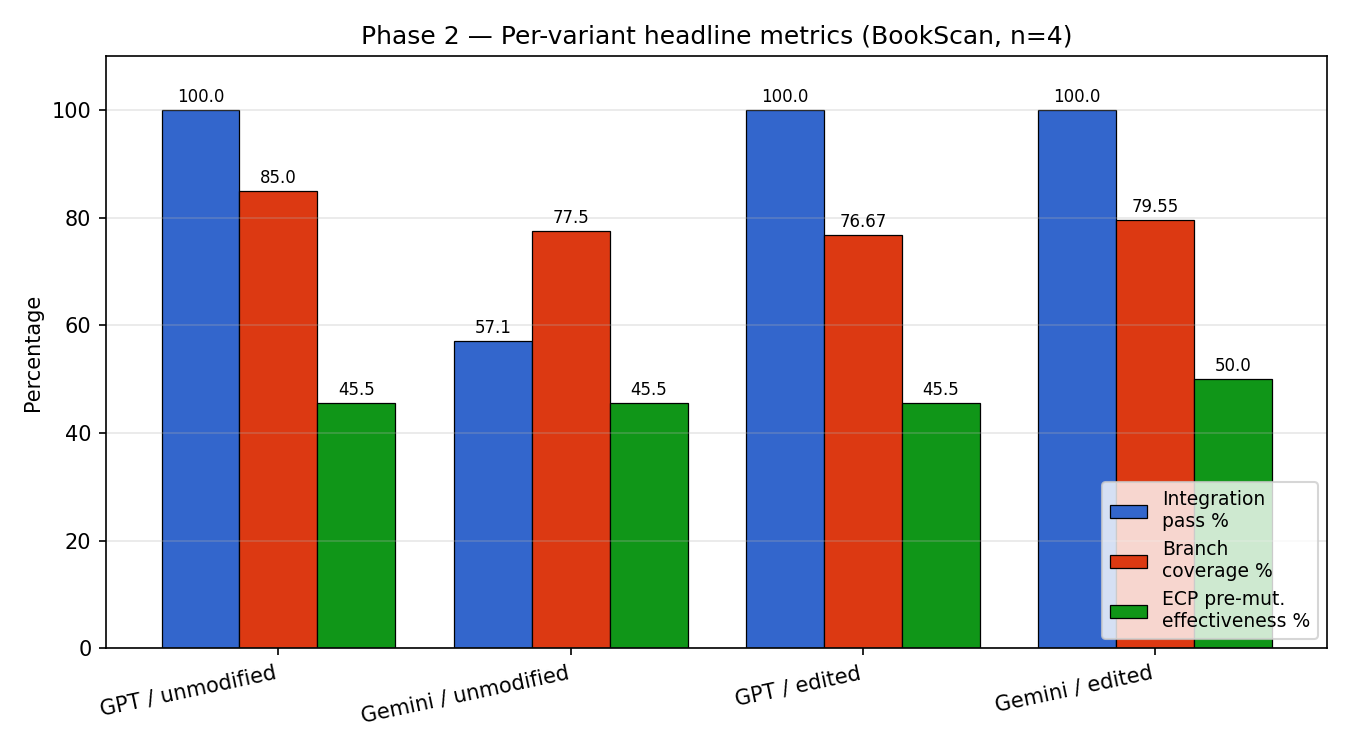
\includegraphics[width=0.95\textwidth]{figures/phase2_comparison.png}
\caption{Phase~2 per-variant headline metrics for the four
BookScan implementations: integration test pass rate, JaCoCo
branch coverage, and ECP pre-mutation effectiveness. The only
visible outlier is Gemini~3.1~Pro under the unmodified prompt
(57\,\% integration pass), where its aspirational test suite
exposes the variant's MixedCase miss and substring-of-longer-
word defects.}
\label{fig:p2comparison}
\end{figure*}

\begin{figure*}[!t]
\centering
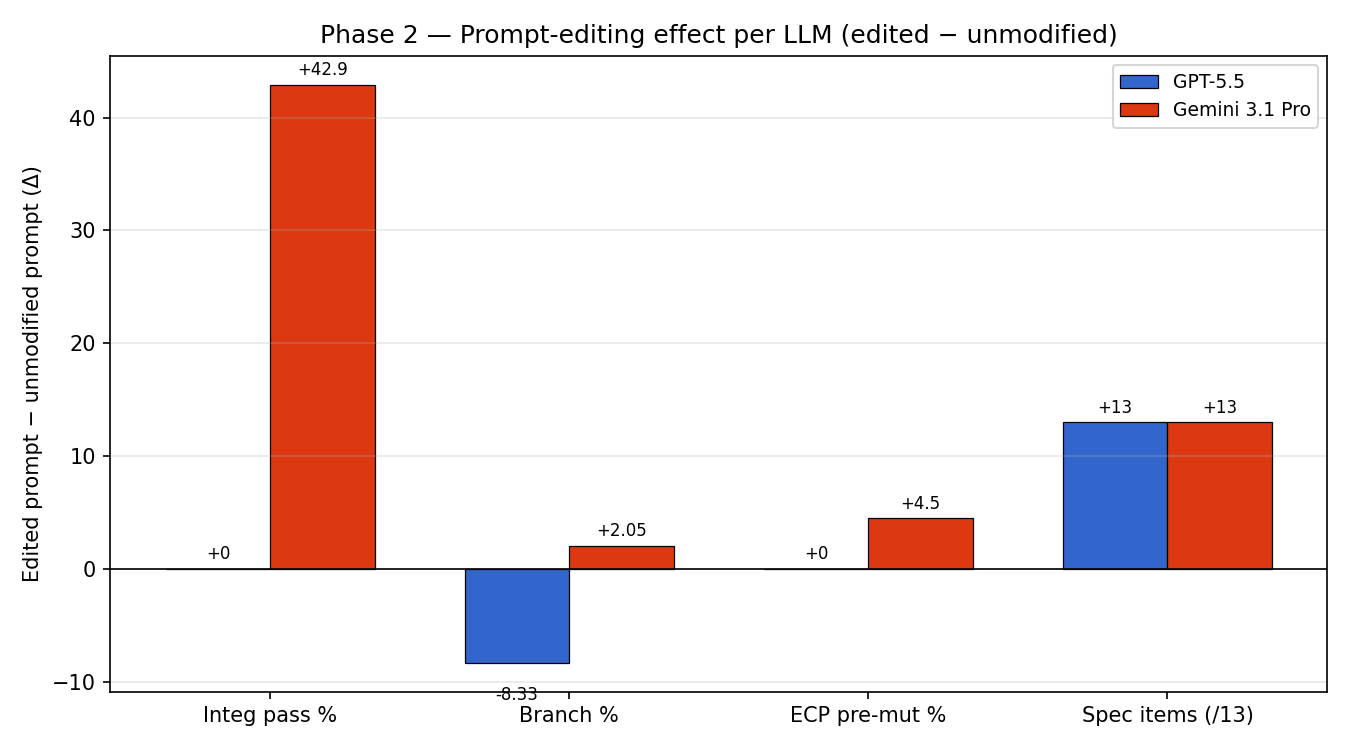
\includegraphics[width=0.95\textwidth]{figures/phase2_prompt_effect.png}
\caption{Phase~2 prompt-editing effect per LLM: bars show
edited-minus-unmodified delta for four headline metrics. Both
LLMs go $0/13 \rightarrow 13/13$ on spec items met; Gemini
gains $+42.9$\,pp on integration pass rate; both LLMs lose a
few branch-coverage percentage points purely as a denominator
effect (the edited variants ship 30\,\% more branches).}
\label{fig:p2effect}
\end{figure*}

\subsection{Integration Failure Analysis}
\label{sec:p2failures}

The Phase 2 BookScan class exposed two qualitatively different
failure modes that no Phase 1 task could have surfaced. First,
the \emph{wrong helper composition rule} anti-pattern: both
unmodified variants called \texttt{flipCase} correctly in
isolation, but composed it with \texttt{howManyTimes} in a
pattern that does not implement case-folded matching (GPT
cancels two flips into a no-op via
\texttt{flipCase(flipCase(x))}; Gemini sums two literal
searches and misses MixedCase variants like ``The''). Second,
the \emph{missing word-boundary invariant}: Gemini's unmodified
variant calls \texttt{howManyTimes} on raw line text, so the
target word ``cat'' matches inside ``concatenate'' and the
target ``a'' matches inside ``have''. A single integration
defect therefore surfaces in two independently-authored test
cases at very different word lengths, which would not happen
with a single-method HumanEval task. The edited prompt
eliminated both classes categorically by (a)~pinning
\texttt{flipCase} to a normalisation role and (b)~requiring a
delimiter-wrapped \texttt{howManyTimes} call site. Both edited
variants produced implementations that pass every Step-6
integration assertion and every Step-9 mutation assertion. A
third anti-pattern, \emph{underspecified contract $\rightarrow$
divergent choices}, accounts for the remaining SPEC-DIVERGENCE
rows (line-list de-duplication in both unmodified variants;
digits and non-ASCII letters as word characters in GPT's
unmodified variant); the full per-failure trace with helper-
call traces and source line citations is in
\texttt{bookscan/reports/failure\_analysis.md}.

\subsection{Refactoring Loop}
\label{sec:p2refactor}

Phase~1's refactoring step never fired; Phase~2 also leaves it
as a deliberate no-op. The three integration test failures in
\texttt{llm\_b/unmodified} are the dependent variable of the
unmodified-vs-edited comparison the brief asks for.
Regenerating that variant with a corrective prompt that names
the failing inputs would yield a v2 closer to the edited
variant, which would erase the SPEC-DIVERGENCE evidence Steps
3--9 were built to collect. We therefore preserve the
unmodified variant unchanged and document the refactoring loop
as deferred-by-design, with a corrective-prompt skeleton
recorded in \texttt{phase2.md} Step~10 for future iterations.

\section{Conclusion}
\label{sec:conclusion}

We applied a single semi-agentic pipeline to two pre-trained
LLMs (GPT-5.5 and Gemini~3.1~Pro) across two phases. Phase~1
covered 30 HumanEval-Java single-method tasks; both LLMs
produced functionally correct code on every task and JaCoCo
branch coverage reached 99.87\,\% after the improvement pass,
yet ECP/BVA rated 27 of 30 base suites below \emph{High}
effectiveness, motivating 30 mutation-based black-box suites.
Phase~2 extended the same instrumentation to a multi-method
\texttt{BookScan} class. A $2 \times 2$ prompt-by-LLM factorial
showed the central effect we set out to measure:
\emph{both LLMs go from 0/13 to 13/13 spec items met under the
edited prompt, and the three integration test failures observed
under the unmodified prompt drop to zero}. JaCoCo branch
coverage averaged 79.68\,\% on the four BookScan variants;
JNose-guided inspection flagged 0 of 81 individual assertions
for Assertion Roulette, versus 30 of 30 in Phase~1's base
suites, because the Phase~2 test-generation prompt explicitly
required failure messages. The six observed integration-failure
modes consolidate to three anti-patterns (wrong helper
composition rule, missing word-boundary invariant,
underspecified contract) that all originate in the unmodified
prompt's gaps and that the edited prompt's explicit contract
eliminates entirely.

The principal recommendation, consistent across both phases, is
to pair JaCoCo (or any branch-coverage tool) with an explicit
ECP/BVA scoring rubric written \emph{before} the LLM is
consulted, and to pin the integration contract --- input shape,
output shape, edge cases, helper roles --- in the prompt
itself. Either change alone shifts a metric or two; the
combination drives the integration-failure class to zero on
both LLMs without sacrificing functional correctness on the
underlying helper methods.

The full pipeline, prompts, generated code, tests, JaCoCo
reports, ECP tables, mutation suites, smell metrics, and
per-step interaction logs are available in the project
repository at\\
\url{https://github.com/itu-itis22-yesilf21/software_quality_0}.\\
The \texttt{phase2} branch contains the Phase~2 work and the
\texttt{gemini} branch is the Phase~1 snapshot; both feed
\texttt{main} once the Phase~2 work is merged.

\section*{Acknowledgments}
All three authors contributed equally to the project;
per-step responsibilities are recorded in the repository
commit history and summarised below.

\subsubsection*{Phase 1 duty split}
\begin{itemize}
    \item \emph{Kutay Murat Kasman}: prompt selection, GPT-5.5
    code generation, base-test adaptation, JaCoCo configuration.
    \item \emph{Furkan Bilal Ye\c{s}il}: Gemini~3.1~Pro code
    generation, JUnit~5 test scaffolding, branch-coverage
    analysis, improved-test refactoring.
    \item \emph{Ahmet \c{C}avdar}: ECP/BVA tables, black-box
    mutation suites, test-smell inspection, Phase~1 report
    writing.
\end{itemize}

\subsubsection*{Phase 2 duty split}
\begin{itemize}
    \item \emph{Kutay Murat Kasman}: BookScan unmodified-prompt
    design, GPT-5.5 Runs 5.1 / 5.3, \texttt{run\_smoke.py} and
    \texttt{run\_integration.py} orchestrators, Step~4 and
    Step~6 analyses.
    \item \emph{Furkan Bilal Ye\c{s}il}: BookScan edited-prompt
    design, Gemini~3.1~Pro Runs 5.2 / 5.4, JaCoCo coverage
    orchestrator \texttt{run\_coverage.py},
    \texttt{run\_black\_box.py} runner, Step~7 and Step~9
    coverage / mutation analyses.
    \item \emph{Ahmet \c{C}avdar}: canonical ECP/BVA table for
    BookScan, four \texttt{BookScanBlackBoxTest.java} suites
    with the SPEC-DIVERGENCE inventory,
    \texttt{analyze\_test\_smells.py} and \texttt{make\_comparison.py},
    failure analysis writeup, Phase~2 report extension.
\end{itemize}

We acknowledge the use of two pre-trained LLMs (GPT-5.5 and
Gemini~3.1~Pro) as artefact generators; all generated
artefacts and the prompts used to obtain them are logged in
\texttt{gemini\_process/logs/code\_generation\_log.md} (Phase~1)
and in \texttt{bookscan/logs/} (Phase~2), and the commit
history records each pipeline step with a step-tagged message
of the form \texttt{Phase~N / Step~M: ...}. The literature
review section (Section~\ref{sec:bg}) was written by the
authors directly from the cited papers; no LLM tool was used
to generate that section. We thank the BLG~475E course staff
for the project specification.

\bibliographystyle{IEEEtran}
\bibliography{references}

\end{document}
